\documentclass[preview]{standalone}
\usepackage{tikz}
\usepackage{physics2}
\usetikzlibrary{decorations.pathmorphing, shapes.geometric}

\RequirePackage{amsmath,amsfonts,amssymb}
% Definición de colores personalizados
\definecolor{primaryColor}{RGB}{20,45,105} % color primario
\definecolor{secondaryColor}{RGB}{0,100,160} % Color secundario

\begin{document}
            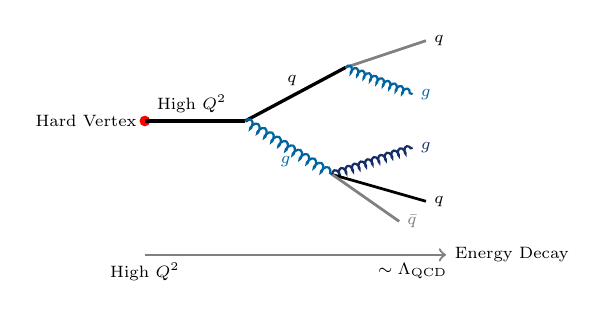
\begin{tikzpicture}[scale=0.85, transform shape]
                % Raíz de la colisión
                \coordinate (V0) at (0,0);
                \fill[red] (V0) circle (0.08);
                \node[left, black] at (V0) {\scriptsize Hard Vertex};
                
                % Línea del Quark inicial
                \draw[line width=1.5pt] (V0) -- (1.5,0);
                \node[above] at (0.7,0) {\scriptsize High $Q^2$};
                \coordinate (V1) at (1.5,0);
                
                % Primera ramificación: q -> q + g
                \draw[line width=1.2pt] (V1) -- (3.0,0.8);
                \draw[thick, secondaryColor, decoration={coil, amplitude=1.5pt, segment length=3pt}, decorate] (V1) -- (2.8,-0.8);
                \coordinate (V2) at (3.0,0.8);
                \coordinate (V3) at (2.8,-0.8);
                \node[above] at (2.2,0.4) {\scriptsize $q$};
                \node[below, secondaryColor] at (2.1,-0.4) {\scriptsize $g$};
                
                % Segunda generación de ramificación
                \draw[line width=1pt, gray] (V2) -- (4.2,1.2);
                \node[right, black] at (4.2,1.2) {\scriptsize $q$};
                
                \draw[thick, secondaryColor, decoration={coil, amplitude=1.2pt, segment length=2.5pt}, decorate] (V2) -- (4.0,0.4);
                \node[right, secondaryColor] at (4.0,0.4) {\scriptsize $g$};
                
                \draw[thick, primaryColor, decoration={coil, amplitude=1.2pt, segment length=2.5pt}, decorate] (V3) -- (4.0,-0.4);
                \node[right, primaryColor] at (4.0,-0.4) {\scriptsize $g$};
                
                \draw[line width=1pt] (V3) -- (4.2,-1.2);
                \node[right] at (4.2,-1.2) {\scriptsize $q$};
                
                \draw[line width=1pt, gray] (V3) -- (3.8,-1.5);
                \node[right, gray] at (3.8,-1.5) {\scriptsize $\bar{q}$};
                
                % Eje de Escala de Energía (Evolución)
                \draw[->, thick, gray] (0,-2.0) -- (4.5,-2.0) node[right, black] {\scriptsize Energy Decay};
                \node[below] at (0,-2.0) {\scriptsize High $Q^2$};
                \node[below] at (4,-2.0) {\scriptsize $\sim \Lambda_{\text{QCD}}$};
            \end{tikzpicture}


\end{document}